\subsection{Entorno}

Algunas de las características importantes del entorno en el que se realizaron las medidas son:
\begin{itemize}\tightlist
  \item Procesador: Intel core i5
  \item OS: Lubuntu 19.10
  \item Shell: Bash 3.2
\end{itemize}

\subsection{Metodología}

Todas las implementaciones
\footnote{Código disponible en
\url{https://github.com/savargasqu/2020-I_Sistemas_operativos/tree/master/IPC_time_measurements}}
usan procesos emparentados,
excepto la implementación de paso de mensajes por \emph{sockets}.
Los datos que se transmiten entre procesos son enteros aleatorios.
El número de enteros que han de ser transmitidos pasa como un argumento de linea de comando para cada proceso.
En todos los casos se escogió transmitir multiplos de 25,
dado que un dato de tipo \texttt{int} ocupa 4 bytes en esta arquitectura.
Así, tenemos $250 \times 4 \text{bytes} = 1 \text{kB}$, y así sucesivamente,
aproximando los tamaños propuestos.

La medidas de tiempo se realizaron con un \emph{script} de Bash \texttt{exec\_times\_tester.sh}.
El tiempo de cada ejecución se midió usando el programa \texttt{time},
y se redirigió la salida a un archivo de texto.
Los resultados de este archivo se copiaron a un \emph{script} de Python,
para hacer una gráfica usando la biblioteca Matplotlib.

\hypertarget{resultados}{%
\subsection{Resultados}\label{resultados}}

\begin{figure}
\centering
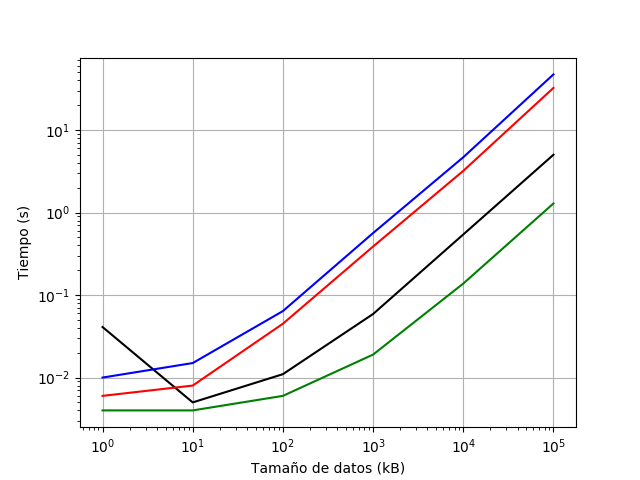
\includegraphics[scale=0.8]{img/results_graph.png}
\caption{Resultados de medición de tiempo para diferentes
IPC}
\end{figure}

En la figura 1. se muestran los resultados de ejecución del
método de memoria compartida en verde;
el método de archivos compartidos en negro;
el método de \emph{pipes} en rojo y
por último el método de \emph{sockets} en azul.

Podemos ver que en escala logarítmica, los resultados aproximan rectas paralelas,
lo que significa que cada método es magnitudes de veces más lento que el anterior.

Se puede ver que para datos más pesados,
la memoria compartida es, de lejos, el método de comunicación más veloz.
Después se encuentra el método de archivos compartidos.
En la prueba este tiene un pésimo desempeño en la primera muestra,
esto se debe a que la operación más costosa es la misma creación del archivo.
Para las muestras siguientes, se comporta de manera similar a los demás IPC,
aunque con un resultado mejor de lo esperado. Es posible que la forma en la que se realizó
la implementación de cada IPC pudo haber favorecido este resultado.
En general, los datos se transmitían uno a uno, no en arreglos,
por lo que un archivo podría ser más rápido que un \emph{pipe} que nunca llena su buffer.
Los métodos de \emph{pipes} y \emph{sockets}, como se esperaba, son más lentos.
Un sobrecosto por su seguridad y facilidad de componer rutas de datos entre
procesos no emparentados.

